\documentclass[12pt,a4paper]{article}
\usepackage[utf8]{inputenc}
\usepackage{hyperref}
\hypersetup{pdfborder={0 0 0}}
\usepackage[frenchb]{babel}
\usepackage[T1]{fontenc}
\usepackage{lmodern}
\usepackage{graphicx}
\usepackage{setspace}
\usepackage{float}
\usepackage[left=2cm,right=2cm,top=2cm,bottom=2cm]{geometry}
\usepackage[center]{caption}
\usepackage{listings}
\usepackage{numprint}
\usepackage{color}
\usepackage{fancyhdr}
\usepackage{soul}
\usepackage{enumitem}
%\newlist{arrowlist}{itemize}{1}
%\setlist[arrowlist]{label=$\Rightarrow$}
\pagestyle{fancy}


\author{J. \textsc{Chaumont} \and P. \textsc{Gourrinchas} \and \textsc{A. Hanriat} \and \textsc{F. Monjalet}}
\title{RE315- Sécurité des Réseaux\\Laptop}

\fancyhead[L]{Sécurité des Réseaux}
\fancyhead[R]{Laptop}

\def\vspaceheight{0.5cm}
\setlength{\headheight}{15pt}

\definecolor{cblue}{RGB}{0,135,195}
\definecolor{cgreen}{RGB}{0,153,0}
\definecolor{cred}{RGB}{255,0,0}

\lstset{
  frame=single,
  keywordstyle=\color{cblue},
  commentstyle=\color{cgreen} \footnotesize,
  stringstyle=\color{cred},
  basicstyle=\footnotesize,
  numbers=left,
  numbersep=5pt,
  tabsize=4
}


\begin{document}


%%%%%%%% Page de couverture %%%%%%%%
\thispagestyle{empty}
\begin{center}

\LARGE{\textsc{RE315 - Sécurité des Réseaux}}\\[0.8cm]
\Large{\textsc{Projet Laptop}}

\vspace*{0.5cm}

\begin{figure}[H]
	\begin{center}
		
\includegraphics[width=200px]{img/logo.jpg}
	\end{center}
\end{figure}

\vspace*{0.3cm}
\Large{J. \textsc{Chaumont}\ \ \ P. \textsc{Gourinchas}\ \ \ \textsc{A. Hanriat}\ \ \ \textsc{F. Monjalet}}\\
\vspace*{1cm}
\large{27/01/2014}



\end{center}

\clearpage
\tableofcontents
\clearpage


\section*{Introduction}
\addcontentsline{toc}{section}{Introduction}

L'explosion des ventes de matériels informatiques nomades, au détriment des stations de travail fixes par exemple, est un bon indicateur des tendances actuelles. Encouragé par l'autonomie croissante des batteries, l'expansion des réseaux mobiles hauts débits ainsi que par la puissance des appareils, le nomadisme numérique est bien plus qu'un effet de mode, et ce, autant pour les loisirs que pour le monde professionnel. En effet, ces dernières années ont vu apparaître le \textit{Bring Your Own Device}, c'est-à-dire le fait qu'un employé utilise ses terminaux personnels dans le cadre de son travail.

Ce constat a certes des côtés positifs en matière de confort d'utilisation: n'importe qui peut être connecté à Internet où qu'il soit, profiter de son ordinateur personnel au travail, et ne plus avoir à systématiquement changer d'appareil en fonction des tâches à réaliser. C'est néanmoins au niveau de la sécurité que se situe la partie la plus inquiétante de ce phénomène. En effet, si un appareil personnel est autorisé à contenir les données d'une entreprise, comment s'assurer de la sécurisation de celui-ci puisqu'il ne relève pas de la juridiction de l'employeur ? 

Par exemple, comment garantir la sécurité des données stockées sur un appareil mobile lorsque celui-ci est volé ? Cette question est loin d'être à prendre à la légère, au vu des chiffres publiés: \numprint{775000} vols de smartphones déclarés en France en 2010\footnote{\url{http://www.inhesj.fr/}}, ou encore 750 vols quotidiens d'ordinateurs portables rien qu'à l'aéroport Charles de Gaulle\footnote{\url{http://www.ponemon.org/}}. Il est à noter que ce point vise aussi bien à protéger les données confidentielles d'entreprise que les données personnelles de l'utilisateur.

La principale réponse à cette question est sans nul doute le chiffrement des disques durs. Il existe aujourd'hui de nombreuses solutions --- commerciales comme libres --- permettant à quiconque de chiffrer ses données afin de rendre impossible l'utilisation de l'appareil sans la connaissance du mot de passe.\\

S'inscrivant dans ce thème, l'objectif du projet était de trouver et d'implémenter des moyens visant à contourner différentes solutions de chiffrement utilisées aujourd'hui. Les attaques ici présentées consistent, le plus souvent, à infecter le secteur de démarrage des machines pour leaker localement ou via le réseau le mot de passe, voir la clé de chiffrement protégeant le disque.


\newpage
\section{Le chiffrement sous Linux avec \texttt{LUKS}}

\subsection{Présentation}

LUKS\footnote{Linux Unified Key Setup} est une spécification de chiffrement de disque dur dont la première version remonte à 2005. L'objectif était de proposer un standard documenté et multi-plateformes (malgré ce que son nom semble indiquer). Sa dernière version en date remonte à 2011\footnote{\url{http://wiki.cryptsetup.googlecode.com/git/LUKS-standard/on-disk-format.pdf}}. C'est ce système qui est utilisé par défaut dans de nombreuses distributions Linux pour le chiffrement de partitions et/ou de disques entiers, même si les implémentations peuvent varier.

Le système est relativement simple. L'utilisateur est seul possesseur d'un mot de passe. Celui-ci est demandée au démarrage de l'ordinateur et sert à déverrouiller la véritable clé de chiffrement : si le mot de passe est correct, alors la clé sera retrouvée et permettra le déchiffrement à la volée du disque chiffré. Si le mot de passe est faux, le système peut le détecter et le redemander.

\begin{figure}[H]
	\centering
        % FIXME, ce schéma est un peu faux, LUKS ne déchiffre pas la
        % partition, il la monte de telle manière que lorsqu'elle est accédée,
        % les données sont déchiffrées à la volée.
        
        % ANSWER modifié
	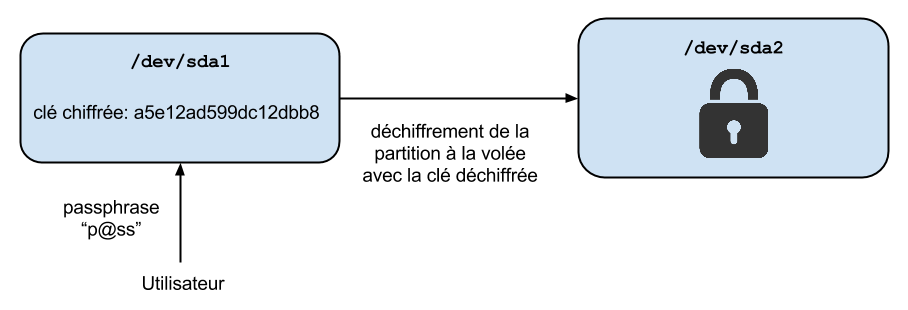
\includegraphics[width=400px]{img/luks_principe.png}
	\caption{Principe de fonctionnement simplifié de LUKS}
\end{figure}

Dans un linux chiffré avec dm-crypt (respectant la spécification LUKS), il y a une partition de boot non chiffrée contenant un \texttt{initrd}. Il s'agit d'un OS linux minimal servant à réaliser le boot du vrai linux. C'est aussi lors de l'exécution de cet \texttt{initrd} que le mot de passe est demandé et que la partition chiffrée est montée de manière à être déchiffrée à la volée avec la bonne clé.

\begin{figure}[H]
	\centering
	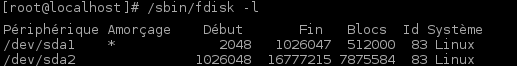
\includegraphics[width=400px]{img/luks_fdisk.png}
	\caption{\texttt{fdisk} indique la présence de deux partitions : la première est la partition de démarrage (elle est en clair), tandis que la seconde contient les données chiffrées}
\end{figure}

\subsection{Principe de l'attaque}

Il s'agit d'infecter l'\texttt{initrd} présent sur la partition de boot de la
machine pour intercepter le mot de passe.
%Au démarrage de l'ordinateur, celui-ci se lance sur une partition \textit{minimale} ne contenant qu'une image de noyau Linux. Elle contient cependant le nécessaire pour demander à l'utilisateur son mot de passe afin de débloquer la clé de chiffrement et ainsi déchiffrer la partition contenant le reste du système.


%L'idée est donc de corrompre la partition de démarrage afin de récupérer le
%mot de passe entré par l'utilisateur.
Le seul pré-requis est d'avoir un accès root à la machine cible, que ce soit
par un accès physique (via un OS bootable, un boot en single user ou autre
astuce) ou non. Notre hypothèse de travail se base sur le principe des attaques
dites \textit{evil maid}. Ce nom imagé fait référence aux attaques pour
lesquelles l'attaquant peut bénéficier d'un accès matériel à la cible de
manière discrète et si possible répétée (d'où la référence à une femme de
chambre dans un hôtel). Dans les attaques de type \textit{evil maid}, on
considère même une personne ayant des connaissances en informatique
potentiellement faible.

L'attaque se divise en deux temps :
\begin{enumerate}
    \item Intercepter le mot de passe.
    \item Le communiquer à l'attaquant.
\end{enumerate}

La communication à l'attaquant peut se faire via internet (on supposera qu'un
Laptop bénéficie d'un accès régulier à internet), ou par stockage discret
localement, puis récupération lors d'un deuxième accès à la machine
(potentiellement au moment du vol de données).

\subsection{Implémentation sur Debian}
\subsubsection*{Méthodologie}
% Aide d'un site
% Écriture à la main de l'attaque complète
% Automatisation de l'infection en shell

Nous avons réalisé et testé l'attaque sur Debian Wheezy uniquement, l'attaque
fonctionne certainement sur d'autres versions, mais nous avons préféré nous
concentrer sur l'élaboration d'attaques contre d'autres technologies une fois
celle-ci en place pour un système, l'intérêt étant d'établir des preuves de 
concept et non des attaques efficaces contre le plus de systèmes et de versions
possibles en pratique.

Pour réaliser cette attaque, nous avons procédé en trois temps :
\begin{enumerate}
    \item D'abord de la documentation sur le fonctionnement général de LUKS et
    des attaques existantes. Cette phase de documentation et de recherche a
    impliqué à la fois des recherches documentaires\footnote{notamment le site
    http://www.wzdftpd.net/blog/index.php?post/2009/10/28/44-implementing-the-evil-maid-attack-on-linux-with-luks},
    et des recherches dans les scripts de l'initrd avec entre autres
    \texttt{grep} et \texttt{find} pour identifier les fichiers intéressants.
    Il a ensuite fallu lire et comprendre ces scripts.
    \item Puis la réalisation de l'attaque \og à la main \fg, c'est-à-dire la 
    construction d'un initrd malicieux à partir de l'initrd présent dans la
    partition \texttt{/boot} d'un Debian.
    \item Enfin l'automatisation de l'attaque, réalisée en shell pur, pour 
    l'exercice d'une part, et pour pouvoir tourner sur un Unix bootable minimal
    d'autre part. Le C aurait pu être utilisé, mais la puissance des commandes
    Unix a été préférée. Les langages de type python ont été exclus à cause du
    critère de minimalité du système à partir duquel l'attaque sera réalisée.
\end{enumerate}


\subsubsection*{Réalisation}
Les concepts de la réalisation de cette attaque sont très simples, sa réalisation
en shell a été, quant à elle, plus délicate. Nous ne détaillerons pas réellement
l'écriture du code, puisqu'il est disponible dans les sources du projet.

L'objectif de l'infection est ici d'intercepter le mot de passe et de le faire
remonter jusqu'au système Linux (qui est protégé par le chiffrement) pour qu'il
puisse être \textit{leaké} via internet.

Les étapes de l'infection sont les suivantes :
\begin{enumerate}
    \item Trouver toutes les partitions bootables.
    \item Essayer de les infecter. Si la partition ne correspond pas à un /boot,
    l'infection retournera un code d'erreur et il suffira de tenter l'infection
    sur la partition suivante : soit la partition n'est pas de la forme cherchée,
    soit le script n'est pas capable de l'infecter correctement.
    \item Monter la partition, trouver et décompresser le ou les initrd. Le
    script essaiera d'infecter chacun d'entre eux.
    \item Trouver le script \texttt{cryptroot} (probablement dans
    \texttt{/scripts/local-top}), trouver et modifier la partie qui demande le
    mot de passe et le passe au programme mettant en place le déchiffrement à la
    volée, puis la changer pour écrire le mot de passe à un endroit du système
    de ficher temporaire du initrd. Pour cet exemple, nous avons choisi le path
    \texttt{/dev/.cryptpass}, car \texttt{/dev} est concervé lors du montage
    du vrai système de fichiers, cela a donc facilité le développement et le
    debug du programme.
    \item Mofifier le script \texttt{init} pour qu'il monte la partition du
    système en \textit{read-write} et non en \textit{read-only}.
    \item Modifier le script \texttt{init} pour qu'il :
    \begin{itemize}
        \item Lise le mot de passe là où il a été stocké.
        \item Supprime le fichier qui contenait le mot de passe (pour plus de 
        discrétion).
        \item Insère à la fin du rc.local du système un script qui envoie le mot
        de passe sur internet et se supprime du rc.local une fois que c'est fait.
        Le détail et la critique de la manière d'envoyer sur internet sera faite
        plus loin.
    \end{itemize}
    \item Recompresser l'initrd et le remettre au bon endroit avec le bon nom.
\end{enumerate}

À la fin de cette infection, à chaque boot du Debian, le mot de passe sera
récupéré et envoyé sur internet.

L'envoi sur internet consiste en une simple requête GET sur une URL que nous
avons mis en place, qui permet de mémoriser un argument de la requête. C'est une
version simpliste, nous aurions pu envisager le post sur un compte twitter ou
utiliser un autre type de serveur permettant de récupérer de l'information de
manière anonyme. Nous n'avons pas cherché à mettre l'accent sur la solidité de
la méthode d'envoi sur le net, le tout était de démontrer que cela était
facilement possible.

Nous avons utilisé netcat pour l'envoi de la requête, l'idéal aurait peut-être
été de tester la présence d'un certain nombre d'utilitaires sur la machine et
choisir l'un d'entre eux (netcat, telnet...), ou d'embarquer notre propre
utilitaire.

\subsubsection*{Conclusion sur l'attaque}

En réalisant cette attaque, nous avons pu voir à quelle point il pouvait être
facile de compromettre un système, même chiffré en ayant juste un accès physique
ou root à la machine (un accès root est suffisant pour réaliser cette attaque).
Sur les systèmes chiffrés avec LUKS, il est même relativement facile de récupérer
la clé de chiffrement elle-même, puisqu'il s'agit simplement d'exécuter une
commande puis de fournir le mot de passe actuel (qui est en notre possession). Il 
suffit de parser la sortie de cette commande pour récupérer la clé. Nous ne 
l'avons pas fait pour passer plus de temps sur d'autres sujets, mais le réaliser
serait encore une fois peu difficile en théorie (et en pratique).

En revanche, les limites de cette attaque, comme de toute attaque sont des
possibles problèmes de robustesse aux changements de noms de variable, de forme
de code. Ces problèmes sont presques inévitables, mais rendent l'infection
fragile.

Il est bon de noter que cette attaque remonte jusqu'au système et permet
d'exécuter du code arbitraire en root sur la machine (via rc.local pour notre 
cas, mais tout est accessible), et d'avoir accès à l'intégralité du système de
fichiers en clair. Il est donc possible d'introduire n'importe quelle backdoor,
rootkit, keylogger dans le système, et même de sortir des données du système sans
avoir un nouvel accès physique.

\subsection{Implémentation sur Fedora}

Fedora diffère de Debian sur de nombreux points. L'une de ces différences est l'utilisation de \texttt{systemd} par Fedora, alors que Debian utilise par défaut le démon \texttt{init} de \textit{System V}. C'est néanmoins une distribution très utilisée, et il était donc intéressant de reproduire l'attaque sur celle-ci. La principale différence avec l'attaque faite sur Debian est que la partie intéressante de l'image \texttt{initramfs} (qui remplace le \texttt{initrd} de Debian) n'est pas un simple script shell, mais un exécutable binaire.

Sur le principe, l'attaque reste la même : décompresser l'image \texttt{initramfs}, trouver et patcher le fichier sensible se trouvant à l'intérieur, puis reconstruire l'image pour remplacer l'originale. Ceci étant, l'écriture dans un script étant bien plus simple à réaliser que l'écriture dans un fichier binaire, le choix a été de remplacer directement le fichier de départ par une autre version compilée par nos soins. Les sources de \texttt{systemd} étant en effet disponibles très simplement, il est ensuite relativement facile de modifier le bon fichier C --- en l'occurrence \texttt{cryptsetup.c} --- et de recompiler le tout.

La backdoor insérée dans le code consiste simplement à récupérer le mot de passe entré par l'utilisateur et à le dissimuler dans la partition de démarrage, de sorte qu'il puisse être récupéré par l'attaquant. Pour ce faire, une nouvelle hypothèse de travail a été introduite, qui est que l'ordinateur cible utilise un système de fichiers de type ext4 (ce qui est généralement le cas). Il fallait en effet déterminer un endroit du disque où l'insertion du mot de passe ne gênerait pas le fonctionnement normal de l'appareil, et de tels emplacements dépendent grandement du système de fichiers.

Il se trouve que la structure du ext4 force la création d'un espace de 1024 octets remplis de zéros au début de chaque groupes de blocs. Cet espace n'est en fait utilisé que dans certains cas rarement rencontrés, et son contenu ne change en rien le fonctionnement du système dans le reste des cas\footnote{\url{https://ext4.wiki.kernel.org/index.php/Ext4\_Disk\_Layout\#Layout}}. C'est donc l'endroit idéal, puisque sa taille est amplement suffisante, et son emplacement au tout début de la partition le rend très simple d'accès.

\begin{lstlisting}[language=C]
int fileno = open("/dev/sda1", O_RDWR);
if(fileno != -1) {
	write(fileno, *passwords[0], strlen(*passwords[0]));
	close(fileno);
}
\end{lstlisting}

Il est ensuite aisé de reprendre les scripts écrits pour l'infection de Debian et de les adapter à ce nouveau cas, en ajoutant cette fois un script qui devra s'exécuter lors du deuxième accès de l'attaquant à la machine afin de récupérer le mot de passe et effacer ses traces (on aura pris soin, lors du premier accès, à avoir réalisé une copie du binaire \texttt{systemd-cryptsetup} original pour le remettre à sa place).

\begin{lstlisting}[language=Bash]
# Retrieve the password by copying the first 1024 bytes of the sector
dd bs=1024 count=1 if=/dev/sda1 of=passdump-devsda1
# Erase the password by putting zeros
dd bs=1024 count=1 if=/dev/zero of=/dev/sda1
# Read the password
hexdump -C passdump-devsda1
\end{lstlisting}


\subsubsection*{Les problèmes rencontrés}

Il était initialement prévu de mener l'attaque comme sur Debian en profitant d'un script lancé au démarrage de l'ordinateur pour envoyer le mot de passe sur Internet. Des difficultés ont été rencontrées et nous ont contraint à changer de tactique pour celle qui a finalement été adoptée.

Le problème majeur est le fait que nous n'ayons pas trouvé précisément quels binaires de systemd étaient appelés après montage du système déchiffré. L'autre point était que sur Fedora, le script \texttt{rc.local} utilisé sur Debian n'est par défaut pas pris en charge, et il faut au préalable avoir démarré le service correspondant.

Avec un peu plus de temps, ces problèmes auraient été résolus, mais plutôt que de perdre du temps à tenter de réaliser la même attaque que précédemment, nous avons fais le choix d'essayer une autre méthode.


%\clearpage
\section{TrueCrypt, la solution gratuite et portable}

\subsection{Présentation}

TrueCrypt est un logiciel développé dès 1997 et toujours maintenu; la dernière version remontant à 2012. Bien que sa licence\footnote{\url{http://www.truecrypt.org/legal/license}} ne fasse pas de lui un logiciel libre, son code source est gratuitement distribué\footnote{\url{http://www.truecrypt.org/downloads2}}. Écrit en grande partie en langage C et en assembleur, TrueCrypt est disponible sur les systèmes Windows, Linux et Mac OS X. Parmi les nombreuses fonctionnalités du logiciel, on compte notamment:
\begin{itemize}
	\item Le chiffrement de dossiers
	\item Le chiffrement de partitions
	\item Le chiffrement de disques complets
\end{itemize}

Un type d'attaque ayant été réalisé sur Linux et ne possédant pas de Mac, nous avons choisi de concentrer nos efforts sur TrueCrypt pour Windows. Nous avons également choisi de nous concentrer sur l'attaque d'un disque entièrement chiffré, présentant à première vue plus de défi qu'une attaque présentant une partie d'un file system en clair.

\subsection{Compilation \textit{maison}}

Le premier type d'attaque tentée est celle qui consiste à délivrer à un client un binaire de TrueCrypt infecté. Elle a le gros avantage de ne pas nécessiter d'accès physique avant le vol de données.

Pour cela, nous avons opté pour une recompilation du binaire pour Windows, le code source étant disponible. Malgré le manque flagrant de documentation et la quantité assez impressionnante de logiciels à installer\footnote{\url{http://stackoverflow.com/a/13414137/2679935}} (et pas des plus simples à se procurer), nous sommes finalement parvenus à compiler le code source du programme. Malheureusement, à l'exécution du binaire résultant, nous étions systématiquement confrontés à une erreur de segmentation dont nous n'avons pu trouver l'origine. Nous avons fait le choix de ne pas aller plus loin dans cette méthode, principalement pour deux raisons:
\begin{itemize}
	\item L'installation de TrueCrypt sur Windows requiert des droits système qui déclenchent l'UAC de Windows (à partir de Vista), et sur lequel on peut voir que l'exécutable en question est authentifié comme émanant de la TrueCrypt Foundation. En recompilant nous-même le programme, nous perdons cette signature. Il est bien sûr possible de désactiver l'UAC, mais ce n'est qu'une faible proportion des utilisateurs Windows qui le font.
	\item Le chiffrement de disque dur ou de partition requiert l'installation des pilotes TrueCrypt. Or, Windows n'autorise par défaut l'installation de ces pilotes que parce qu'ils sont signés et reconnus. Là encore, l'utilisateur peut avoir explicitement autorisé son système à installer des pilotes non signés, mais c'est loin d'être le cas général.
\end{itemize}

\begin{figure}[H]
	\centering
	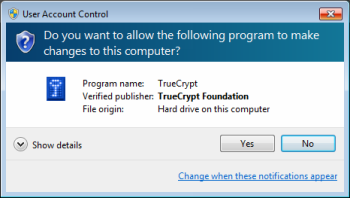
\includegraphics[width=300px]{img/truecrypt_uac.png}
	\caption{L'UAC authentifie la provenance de l'exécutable}
\end{figure}



\subsection{Le phishing au démarrage}

Une autre solution beaucoup plus simple à mettre en place était de falsifier l'écran de demande de mot de passe de TrueCrypt. Pour cela, un simple programme en C a été réalisé à l'aide de la bibliothèque graphique \textit{ncurses}.

\begin{figure}[H]
	\centering
	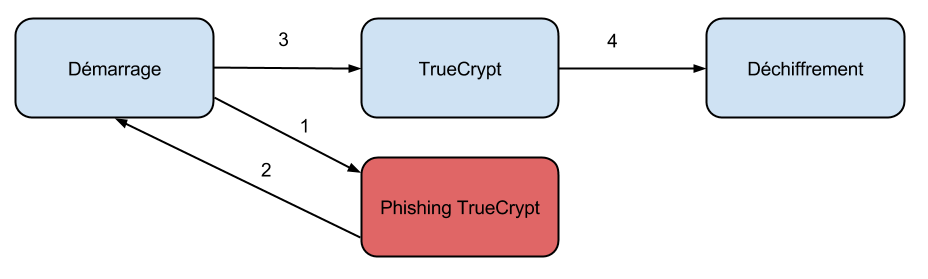
\includegraphics[width=400px]{img/truecrypt_phishing.png}
	\caption{Principe du phishing TrueCrypt}
\end{figure}

Le programme reprend avec soin l'affichage exact de l'écran de démarrage par défaut de TrueCrypt en version 7.1a (la dernière en date), et demande la saisie du mot de passe. L'opération est répétée trois fois avant d'afficher un message d'erreur invitant l'utilisateur à redémarrer sa machine. Entre temps, les mots de passe saisis par l'utilisateur auront été soigneusement stockés en mémoire.

\begin{figure}[H]
        % FIXME L'erreur de TrueCrypt pour un mot de passe raté est plutôt
        % quelque chose du genre "Invalid Password. Retry.", à vérifier !
        
        % ANSWER L'idée était d'afficher un message différent de d'habitude
        % pour "justifier" l'erreur qui apparaît au bout de 3 tentatives.
        % Et ce message d'erreur existe bien:
        % http://www.truecrypt.org/docs/troubleshooting
	\centering
	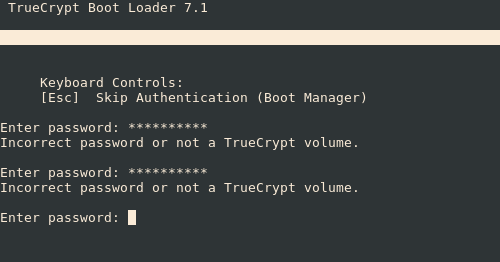
\includegraphics[width=400px]{img/truecrypt_ncurses.png}
	\caption{Affichage du programme de phishing TrueCrypt}
\end{figure}

Pour mettre en place cette attaque, l'idée était d'utiliser la clé USB bootable utilisée pour LUKS, mais en y apportant quelques modifications afin de la rendre la plus \textit{silencieuse} possible: en d'autres termes, pouvoir démarrer sur cette clé sans que la personne devant l'écran ne puisse constater la supercherie.

Cette façon de faire a néanmoins de nombreuses lacunes:
{
\renewcommand{\labelitemii}{$\Rightarrow$}
\begin{itemize}
	\item on suppose un accès physique à la machine cible pour placer la clé USB puis pour la récupérer
	\begin{itemize}
		\item il s'agit là de l'hypothèse de travail pour une attaque \textit{evil maid}
	\end{itemize}
	\item on suppose avoir un accès au BIOS de la machine afin de modifier la séquence de démarrage
	\begin{itemize}
		\item la proportion d'utilisateurs ayant pris soin de mettre un mot de passe à son BIOS est suffisamment faible
	\end{itemize}
	\item on fait confiance à l'utilisateur pour qu'il ne remarque pas la clé branchée sur son port USB
	\begin{itemize}
		\item sur un ordinateur fixe, cette supposition est parfaitement envisageable
		\item elle l'est plus difficilement sur un ordinateur portable, bien qu'on puisse envisager une clé USB enfichable pouvant se cacher derrière une autre légitime (celle de la souris par exemple). Garder la clé non remarquée suffisamment longtemps reste cependant très improbable.
	\end{itemize}
	\item l'utilisateur doit avoir installé la version 7.1a de TrueCrypt et ne pas avoir activé d'options faisant apparaître de nouveaux éléments à l'écran de démarrage (message personnalisé activable)
	\begin{itemize}
		\item la version 7.1a date de février 2012, on peut donc supposer que c'est celle qui est adoptée dans la majorité des cas
		\item quant à l'activation d'options, on peut supposer que celles proposées par défaut sont suffisantes pour la plupart des utilisateurs
	\end{itemize}
	\item on suppose que l'écran d’accueil de TrueCrypt est celui qui doit apparaître en premier
	\begin{itemize}
        % FIXME Faire cohabiter Grub et TrueCrypt est un problème délicat en
        % soi, je pense qu'on peut l'exclure de notre type d'attaque (contre
        % le chiffrement total de disque). TrueCrypt s'installe dans le MBR,
        % si on boot sur ce disque dur, TrueCrypt devra à priori être le premier
        % à apparaître.
		\item cette supposition assez forte rejette par exemple les machines démarrant sur Grub
	\end{itemize}
\end{itemize}
}

Il est cependant à noter que les deux derniers points peuvent être contrés en
se renseignant au préalable sur la cible et en adaptant le programme de
phishing en conséquence.


\subsection{Modification du secteur de boot}

Après examen plus en profondeur du fonctionnement de TrueCrypt, nous avons
choisi d'implémenter une attaque qui consisterait en la modification directe du
code présent dans le secteur d'amorçage.

\subsubsection{Méthodologie}

Pour mener à bien cette attaque, nous avons du commencer par nous renseigner
sur les mécanismes impliqués dans le boot d'une machine sur un disque dur : il
s'agit principalement de l'exécution d'une petite portion de code présente dans le
MBR (premier secteur du disque dur).

En désassemblant ce code (avec IDA), nous avons pu retrouver la source
assembleur correspondante dans les sources de TrueCrypt, contenant des
informations donnant plus de sens au code (évitant par la même occasion de perdre du
temps à reverser le code désassemblé). Il a tout de même fallu se familiariser
avec les diverses interruptions utilisées pour les I/O, ainsi que quelques
spécificités de l'assembleur 16 bits présent dans les MBR.

Une fois la séquence de boot comprise et les fonctions clés repérées (notamment
la fonction AskPassword), nous avions pour projet d'intercepter le mot de passe
entré par l'utilisateur et de le sauvegarder quelque part (sans encore savoir
où).

C'est la découverte de l'implémentation d'une attaque similaire par Johanna
Rutkowska\footnote{Plus d'informations sur
http://theinvisiblethings.blogspot.ch/2009/10/evil-maid-goes-after-truecrypt.html}
(\textit{Evil Maid Goes After TrueCrypt}) qui a accéléré le processus
d'écriture de l'attaque. Le résultat est bel et bien notre production et notre
vision de l'attaque, mais une grande partie du debug été facilitée par la
lecture de l'implémentation de Johanna Rutkowska.

Nous allons maintenant parler plus en profondeur de chaque étape de l'attaque.

\subsubsection{Séquence de boot de TrueCrypt}

La séquence de boot de TrueCrypt est relativement simple, comme le montre la
figure \ref{tc_boot}. Toute la séquence se déroule en mode réel, c'est à dire
en mode 16 bits.

Il est bon de noter que le seul semblant d'OS qui est à la disposition du
programme à ce stade du boot est le BIOS, et les interruptions qu'il propose.
TrueCrypt réimplemente donc un ensemble de fonctions (notamment d'affichage)
utilisant les interruptions disponibles au niveau assembleur.

Les étapes sont les suivantes :
\begin{enumerate}
    \item Le bootloader présent dans le MBR est exécuté, charge le Decompressor
    et le bootloader de TrueCrypt (qui est à ce stade compressé) en RAM. Leurs
    checksums sont vérifiées, et il y a abandon si elles ne sont pas bonnes.
    \item Le decompressor est exécuté, et décompresse le bootloader de
    TrueCrypt.
    \item Si l'étape précédente est réussie, alors le bootloader fraîchement
    décompressé est exécuté. Ceci est réalisé via l'empilement du registre de
    segment \texttt{es}\footnote{en assembleur intel 16bits, le registre
    \texttt{es} est utilisé conjointement à d'autres registres pour simuler un
    adressage sur 20 bits (\texttt{es << 4 + reg}).} (valant 0 ici) et de
    l'adresse du code dans le segment, en l'occurrence \texttt{0x100} puis
    l'exécution d'un \texttt{retf}.
    \item C'est ce bootloader qui demande le mot de passe : 
    c'est donc ici que nous allons agir pour l'intercepter.
\end{enumerate}

\begin{figure}[H]
    \centering
    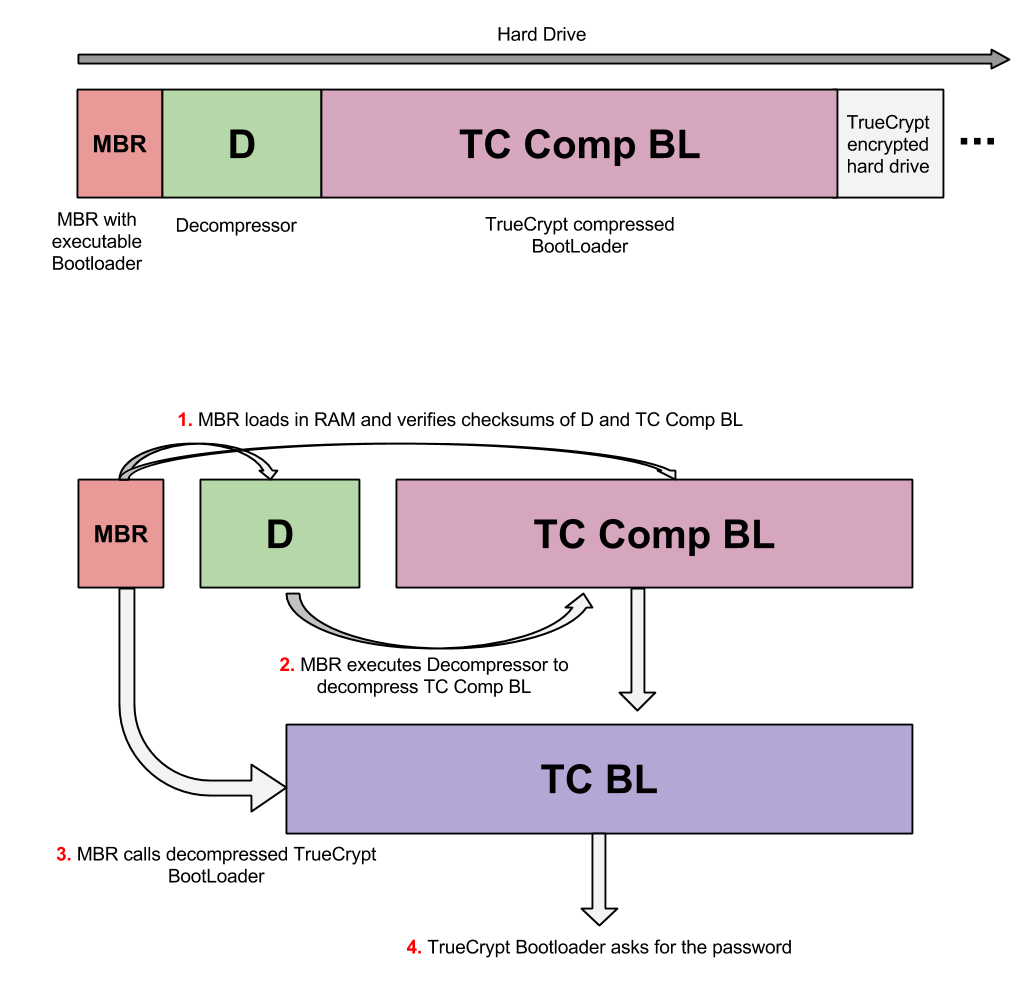
\includegraphics[height=0.5\textheight]{img/tc_boot.png}
    \caption{Séquence de boot (simplifiée) de TrueCrypt}
    \label{tc_boot}
\end{figure}

\subsubsection{Infection du code}

Comme nous avons pu l'identifier précédemment, le mot de passe est récupéré et
utilisé par le bootloader de TrueCrypt, l'idée va donc être de modifier ce
bootloader pour \textit{leaker} le mot de passe.

\paragraph{Obtention du binaire du bootloader}~

Pour obtenir le binaire décompressé et travailler dessus, il faut commencer par
récupérer la version compressée. Pour cela, nous avons repéré, en comparant
le code assembleur source et le code présent dans le MBR après compilation,
les valeurs indiquant depuis quels secteurs du disque dur ce bootloader était
chargé. Cela a permis d'automatiser la récupération du bootloader compressé,
et de s'apercevoir d'un espace vide de quelques secteurs réservé par TrueCrypt,
qui nous servira par la suite.

Pour décompresser le binaire, on peut soit appeler le décompresseur de
TrueCrypt (en l'adaptant à notre environnement de travail), soit noter qu'il
s'agit d'une implémentation de GZip qui a été adaptée au projet. Nous avons
choisi la deuxième solution, et décompressé le code via GZip. Les options de
recompression sont visibles dans le Makefile du secteur de boot (qui utilise
gzip).

Ce binaire exécutable est au format COM, format très simple où il n'y a qu'un
seul segment contenant code et data. Les premiers octets du fichiers sont
directement interprétés comme exécutables.

\paragraph{Isolation du code intéressant}~

TrueCrypt fournissant son code source, il a été facile de repérer la fonction à
cibler : \texttt{AskPassword} (fichier \texttt{BootMain.cpp}), dont le
prototype est le suivant :

\begin{center}
    \texttt{void AskPassword(Password \&password)}
\end{center}

Le choix a été fait (comme dans l'attaque de Johanna Rutkowska) de ne pas
\textit{insérer} du code (entreprise très périlleuse), mais d'ajouter du code
après le binaire. Pour repérer la fonction \texttt{AskPassword} dans le code
décompressé, nous sommes partis des données (les messages affichés dans
AskPassword, faciles à repérer dans le code avec un \texttt{strings -t x \$file
| grep all}) et avons rapidement pu trouver l'endroit où était le code (grâce à
IDA).

Le code appelant \texttt{AskPassword} est facilement trouvable grâce aux
références croisées de IDA.

\paragraph{Man in the middle applicatif}~

L'infection du code repose sur l'idée du Man in the Middle. Pour notre
implémentation, nous avons choisi de suivre la méthode employée par Rutkowska,
mais présenterons plus bas une autre méthode possible. La méthode utilisée
repose sur l'idée d'intercaler un appel à un code arbitraire avant l'appel à 
\texttt{AskPassword} (voir figure \ref{ask_tweak}, qui donne un aperçu de l'état
de la pile lors de l'appel d'\texttt{AskPassword} par notre code inséré).
L'attaque consiste en la séquence d'actions suivante :

\begin{enumerate}
    \item Insérer le code "Man in the Middle" (son contenu est expliqué plus loin)
    à la fin du binaire.
    \begin{itemize}
        \item La première version consistait à écrire le code à la suite de la
        section \texttt{data} du bootloader, mais cela causait des bugs étonnants.
        Il s'avérait que le programme se servait de cet espace (pour le BSS très
        certainement), nous avons fini par trouver (grâce à l'exemple de
        Rutkowska) qu'il existait une variable définissant la taille totale
        nécessaire au programme (0x6F00 nécessaire pour le code, les
        data, le bss et la pile, contre environ 0x4c00 pour code et data
        seulement).
        \item Nous avons placé le code après cette valeur (à l'offset 0x6F00 du
        bootloader décompressé), rempli l'espace non utilisé de 0 (pour que le
        bootloader recompressé ne dépasse pas la taille maximale autorisée). Il
        a ensuite fallu réécrire la constante donnant la taille nécessaire au 
        programme dans le MBR.
    \end{itemize}
    \item L'appel intéressant à \texttt{AskPassword} dans le code est retrouvé
    dans le code binaire au moment de l'infection grâce à la recherche d'une
    chaîne binaire l'identifiant de manière unique (une seule occurrence dans
    le fichier). On aurait pu directement donner l'offset de l'appel, mais on
    considèrera qu'un fichier issu de code C compilé est plus prone à varier
    que le programme en assembleur du bootloader (où des offsets avaient été
    utilisés). Ceci étant, les deux méthodes ont leurs défauts.
    \item Une fois l'appel retrouvé, on a toutes les informations : l'offset de
    l'appel, l'offset d'\texttt{AskPassword} et on connaît l'offset de notre code.
    Il ne reste plus qu'à :
    \begin{itemize}
        \item Faire pointer l'appel à \texttt{AskPassword} vers notre code.
        \item Faire en sorte que le \texttt{call} de notre code pointe vers
        \texttt{AskPassword}.
    \end{itemize}
\end{enumerate}

\paragraph{Récupération et sauvegarde du mot de passe}~

\begin{figure}
    \centering
    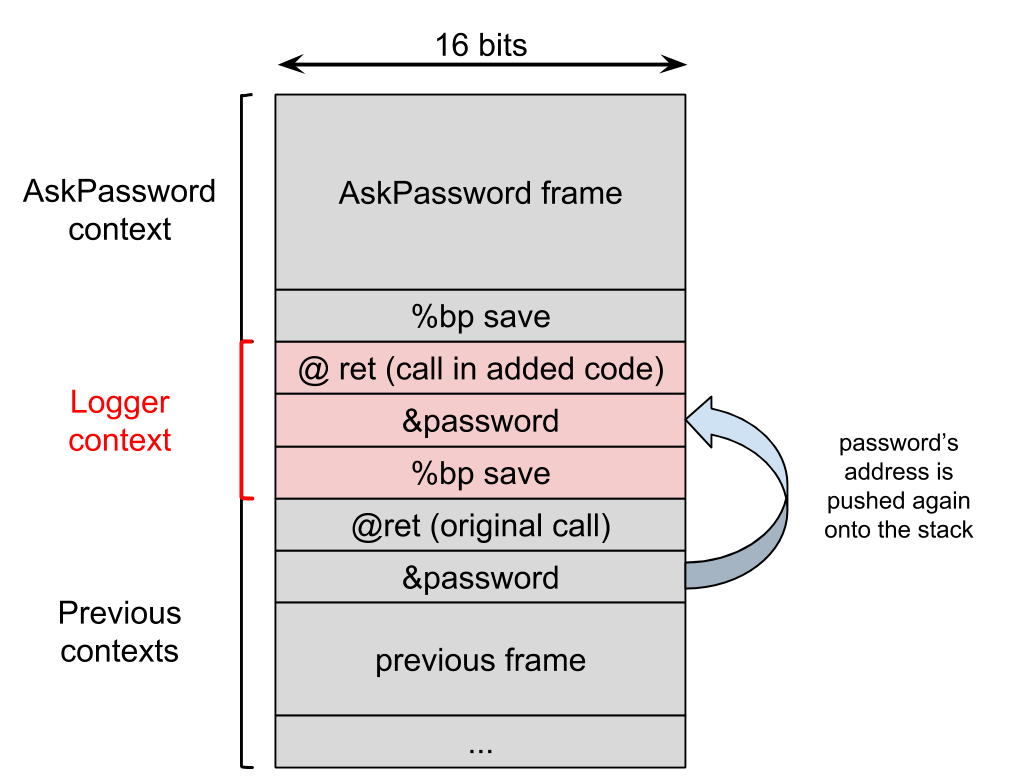
\includegraphics[height=0.3\textheight]{img/pile_tc.png}
    \caption{Vu de l'état de la pile lors de l'appel à \texttt{AskPassword} par
             le code inséré.}
    \label{ask_tweak}
\end{figure}

Pour la récupération du mot de passe, nous avons réutilisé le code assembleur
rédigé par Rutkowska. C'est ce code qui a été ajouté au binaire pour
\texttt{leaker} le mot de passe. Ce bout de code était nommé \og logger \fg, nous
avons gardé le même nom (il s'agit du fichier \texttt{logger.asm}).

Ce code a un fonctionnement très simple : il commence par réempiler l'argument
\texttt{\&password} (la référence sur la variable \texttt{password}, ce qui
correspond en assembleur à son adresse) attendu par \texttt{AskPassword}, puis
appelle cette fonction.  \footnote{Comme expliqué plus haut, l'appel à
\texttt{AskPassword} est patché lors de l'infection, l'adresse pointée par le
call dans le code est fictive.}. Lorsqu'elle est appelée, \texttt{AskPassword}
remplira la structure Password avec le bon contenu, et le code interposé n'aura 
qu'à dumper le contenu de celle-ci.

Le dump de la structure est une question qui peut paraître délicate de prime
abord : aucun système de fichier n'est à notre disposition à ce moment du boot.
Alors où le stocker ?

La réponse que Rutkowska a apporté à la question est simple : sur le disque.
Dans son code, elle utilise l'interruption 0x13 pour les I/O disque pour écrire
dans le secteur 61 (en les numérottant depuis 0).

Surpris par ce chiffre, nous avons décidé de chercher un endroit où nous aurions
une garantie que les données ne seraient pas écrasées. Le lecteur attentif se
souviendra qu'il restait de l'espace non utilisé dans celui que TrueCrypt se 
réserve pour stocker le bootloader compressé. Nous allons donc utiliser le dernier
secteur\footnote{Un secteur fait généralement 512 octets} réservé pour stocker
le mot de passe (l'espace libre est bien supérieur à la taille d'un secteur).
Le bootloader compressé commence au secteur 5 et réserve 57 secteurs (constaté
dans nos tests), 5 + 57 -1 = 61. Le dernier secteur réservé par TrueCrypt est le
numéro 61, d'où le choix de Rutkowska.

Ce nombre n'étant pas nécessairement le même pour toutes les installations (mais
suffisamment souvent le même pour avoir une attaque qui fonctionne souvent), il
aurait été une bonne chose de remplacer également cette valeur au moment de
l'infection par la valeur adaptée à l'installation de TrueCrypt visée. Nous ne
l'avons pas fait pour simplifier l'attaque, mais ça serait une piste
d'amélioration.

La structure contenant le mot de passe est donc tout simplement dumpée sur le
secteur choisi, et il suffira de lire ce secteur lors d'un accès ultérieur au
disque dur pour récupérer le mot de passe. L'hypothèse d'un deuxième accès au
disque dur machine est plus que raisonnable, puisque le but de ce type d'attaque
est de récupérer les données d'un disque chiffré.

\paragraph{Autre méthode}~

Plutôt que de patcher un, ou des appels à AskPassword, on aurait pu envisager
de patcher la fonction elle-même en remplaçant le dernier \texttt{ret} et 
quelques instructions précédentes par un jump sur le code ajouté. Dans le code
ajouté on aurait exécuté les instructions qui ont dû être enlevées de AskPassword
pour faire loger le jump (3 octets en assembleur 16 bits), puis écrit la structure
password sur le disque et enfin fait le \texttt{ret} final.

Cela reviendrait à rajouter du code à \texttt{AskPassword} plutôt que
d'intercepter l'appel. L'adresse de AskPassword peut être trouvé de manière
relativement fiable en trouvant l'une des chaînes affichées par cette fonction
et en cherchant les occurrences de son adresse dans le code.

Nous n'avons pas mis en place cette version car nous avons suivi la ligne
directrice de Rutkowska, mais cela aurait été intéressant à réaliser.


\paragraph{Derniers détails} ~

Après avoir réalisé tout ce processus d'infection, il ne faudra pas oublier de :
\begin{itemize}
    \item Recompresser le bootloader avec les bonnes options (pour que le
    Decompressor le décompresse correctement lors du boot). Ces options sont
    visibles dans le Makefile de la partie Bootloader des sources de TrueCrypt.
    \item Soit recalculer la checksum du bootloader infecté une fois recompressé,
    soit tout simplement la bypasser en remplaçant un \texttt{jz} par un simple
    \texttt{jmp}. Rutkowska a choisi la première option, nous la seconde.
    \item Comme dit plus haut, mettre à jour la taille de la mémoire nécessaire
    à la bonne exécution du bootloader.
\end{itemize}

\subsubsection{Pour aller plus loin...}

On s'aperçoit avec ce type d'attaque que si on peut infecter l'étape de
récupération du mot de passe, rien n'empêche à priori d'infecter les étapes 
suivantes, avec pour objectif d'injecter un rootkit ou une backdoor dans le
système qui est sur le disque chiffré. Ce rootkit pourra donner tous les droits
nécessaires à l'exploration du disque à distance sans même avoir besoin
d'accéder au disque de nouveau.

Cela nécessiterait de se plonger dans le code de TrueCrypt (les sources et les
binaires) plus longtemps pour en comprendre assez le fonctionnement. TrueCrypt
étant maintenu par deux personnes et très, très peu documenté, cette entreprise
n'est pas simple. Il est juste bon de savoir qu'avec du temps et de la motivation,
un tel rootkit serait probablement réalisable.

\subsubsection{Conclusion}

Nous sommes très satisfaits d'avoir pu écrire une attaque de ce type. Même si
nous nous sommes appuyés sur les travaux de Johanna Rutkowska pour certains
aspects de l'implémentation, le résultat est le fruit de notre travail, et
certaines différences dans les choix qui ont été faits en attestent.

Nous n'avons pas récupéré la clé de chiffrement utilisée par TrueCrypt, mais une
fois de plus, en lisant un peu plus le code, et étant donné que nous sommes en 
possession du mot de passe, la clé de chiffrement ne devrait pas être trop 
compliquée à récupérer.

La possibilité (et la facilité) d'une telle attaque contre TrueCrypt, qui est un
programme à la fois Open Source et à très bonne réputation pousse à penser qu'avec
un temps suffisant pour examiner le cas BitLocker, on pourrait construire une
attaque similaire.


%\clearpage
\section{BitLocker pour Windows}

\subsection{Présentation}



%\clearpage
\section{Les autres solutions}

\subsection{Cold Boot Attack}

Quelle que soit la solution logicielle utilisée, la clé de déchiffrement d'un disque finit tôt ou tard par apparaître dans la mémoire vive de l'ordinateur. Même si celle-ci est effacée dès extinction de l'ordinateur, il a été prouvé que les données y figurant pouvaient être récupérées dans les secondes qui suivaient, cette durée pouvant s'étendre à plusieurs minutes en refroidissant les barrettes de mémoire vive\footnote{\textit{Lest We Remember: Cold Boot Attacks on Encryption Keys}, 2008:\\
~~~~~~\url{https://citp.princeton.edu/research/memory/}}.

\begin{figure}[H]
	\centering
	\begin{tabular}{|l|c|c|c|}
	\hline
	Mémoire & Secondes après & \% d'erreurs & \% d'erreurs\\
			& extinction &  à température ambiante & à -50\degre C\\
	\hline
	128Mo SDRAM & 60 & 41 & 0\\
	\cline{2-4} & 300 & 51 & 0.000095\\
	\hline
	256Mo DDR & 120 & 41 & 0.005105\\
	\cline{2-4} & 360 & 42 & 0.00144\\
	\hline
	512Mo DDR & 360 & 50 & 0\\
	\cline{2-4} & 600 & 50 & 0.000036\\
	\hline
	512Mo DDR2 & 40 & 50 & 0.025\\
	\cline{2-4} & 80 & 50 & 0.18\\
	\hline
	\end{tabular}
	\caption{Comparaison de l'efficacité de la \textit{Cold Boot Attack},\textit{Lest We Remember: Cold Boot Attacks on Encryption Keys}, 2008}
\end{figure}

Il serait donc parfaitement envisageable d'ôter la RAM d'un ordinateur venant de s'éteindre, de la refroidir rapidement et d'en récupérer le contenu. Il ne resterait plus ensuite qu'à retrouver la clé de chiffrement parmi les gigaoctets de données\dots


\subsection{Dump de la RAM}

Sur le principe de base de la \textit{Cold Boot Attack}, en supposant un accès root à la machine cible, il est possible de réaliser une copie exacte de la mémoire vive.
Pour réaliser le dump de la ram sans retirer physiquement la RAM de ses slots, nous réalisons une copie via une clef USB.

Une première contrainte est que le fait de charger un OS pour réaliser un dump de la mémoire écrase 
inévitablement une partie des données présentes en RAM. Cet OS se doit donc d'être le plus petit 
possible. 
Une autre contrainte est que depuis la version 2.6, il n'est plus possible de lire librement dans 
/dev/mem. Une première solution consiste à recompiler le noyau en désactivant la sécurité 
empêchant cette action.

%% TODO screenshot make menuconfig

La deuxième solution consiste à charger \texttt{fmem}, un module noyau créant un nouveau fichier 
dans /dev permettant d'accéder à l'ensemble de la mémoire sans aucune limite. Cette solution a pour avantage qu'elle ne nécessite pas la recompilation du noyau.

\begin{lstlisting}[language=Bash]
dd if=/dev/fmem of=/mnt/dump bs=1MB count=4096
\end{lstlisting}

Mais là encore, il reste la difficile étape de retrouver la clé de chiffrement 
parmi l'énorme quantité de données récupérée.


\subsection{Analyse et récupération de la clef de chiffrement via Volatility}
D'après l'ouvrage \texttt{RAM is key}\footnote{http://cryptome.org/0003/RAMisKey.pdf}
le mot de passe se trouve dans l'espace mémoire correspondant au driver de TrueCrypt.
De plus une recherche avec le format [1 byte size][3 null bytes][passphrase][1 null byte]
permet de localiser le mot de passe au sein de l'espace mémoire du driver.


\subsection{La solution de l'acharnement: le brute-force}

Dans le cas où l'attaquant a les ressources en temps et en matériel et que celui-ci souhaite 
ardemment récupérer le contenu chiffré, il est toujours envisageable de déployer une attaque 
par force brute. Le problème intrinsèque au mot de passe est qu'il doit à la fois être 
suffisamment complexe pour qu'il ne puisse pas être trouvé aisément, tout en étant suffisamment 
\textit{simple} pour que l'utilisateur puisse s'en souvenir pour le saisir sans avoir à le noter
à côté de son poste. Même si, par des moyens mémotechniques, on peut envisager l'utilisation de mots
de passe d'une vingtaine de caractères, il est certain que les avancées technologiques finiront tôt 
ou tard par permettre la récupération de mots de passe de cette taille de manière relativement 
rapide.

Il est peut-être donc temps désormais de passer à un autre type d'authentification, 
plus complexe à outrepasser, telle que l'authentification biométrique.




%\clearpage
\section*{Conclusion}
\addcontentsline{toc}{section}{Conclusion}

\section*{Bibliographe}
% TODO BIBLIOGRAPHIE

\end{document}
